%%%%%%%%%%%%%%%%%%%%%%%%%%%%%%%%%%%%%%%%%%%%%%%%%%%%%%%%%%%%%%%%%%%%%%%%%%%%%%%%%%
\begin{frame}[fragile]\frametitle{}
\begin{center}
{\Large Linear Algebra }
\end{center}
\end{frame}

%%%%%%%%%%%%%%%%%%%%%%%%%%%%%%%%%%%%%%%%%%%%%%%%%%%%%%%%%%%%%%%%%%%%%%%%
\begin{frame}[fragile]\frametitle{What's in a name?}
\begin{itemize}
\item ``Algebra'' means, roughly, ``relationship'', between unknown numbers.
\item Without knowing x and y, we can still work out that $(x + y)^2 = x^2 + 2xy + y^2$ 

\item ``Linear Algebra'' means, roughly, ``line-like relationships''.

\item Meaning, not curve like, ie quadratic, cubic, sinusoidal, etc, right? \item Nothing in ``power'' term!!

\item An operation F is linear if scaling inputs scales the output, and adding inputs adds the outputs:

\begin{align*}
    F(ax) &= a.F(x) \\
		F(x+y) &= F(x) + F(y)
\end{align*}

\item When plotted, its a line!!
\end{itemize}

{\tiny (Ref: An Intuitive Guide to Linear Algebra - Better Explained)}
\end{frame}


%%%%%%%%%%%%%%%%%%%%%%%%%%%%%%%%%%%%%%%%%%%%%%%%%%%%%%%%%%%%%%%%%%%%%%%%
\begin{frame}[fragile]\frametitle{Linear Equations}
\begin{itemize}
\item $F(x,y,z) = 3x + 4y + 5z$
\item Whats an example for this?
\item Can you represent this by multiplication of two vectors?
\end{itemize}

{\tiny (Ref: An Intuitive Guide to Linear Algebra - Better Explained)}
\end{frame}

%%%%%%%%%%%%%%%%%%%%%%%%%%%%%%%%%%%%%%%%%%%%%%%%%%%%%%%%%%%%%%%%%%%%%%%%
\begin{frame}[fragile]\frametitle{Basic Entities}
\begin{itemize}
\item Scalars?
\item Vectors?
\item Matrices?
\item Next? (or Whats this called collectively?)
\item Point in n-dimensional space is represented by?
\end{itemize}
\end{frame}



%%%%%%%%%%%%%%%%%%%%%%%%%%%%%%%%%%%%%%%%%%%%%%%%%%%%%%%%%%%
 \begin{frame}[fragile] \frametitle{Landscape: Linear Algebra}

\begin{center}
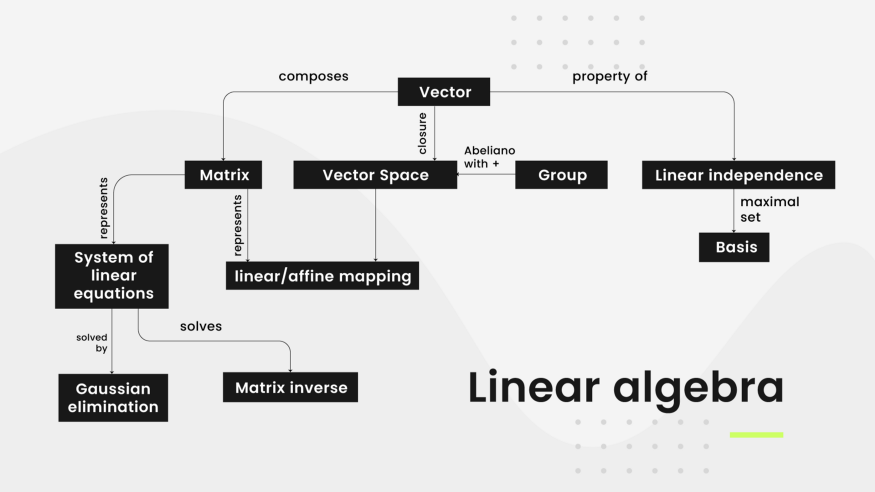
\includegraphics[width=0.9\linewidth,keepaspectratio]{maths4ai1}
\end{center}

{\tiny (Ref: The NOT definitive guide to learning math for machine learning - Favio Vazquez)}

\end{frame}








